\documentclass[10pt]{article}
\usepackage{tmlr}
% Anonymous submission. Use \usepackage[accepted]{tmlr} for the camera-ready
% version and \usepackage[preprint]{tmlr} for a preprint server.

\usepackage{hyperref}
\usepackage{url}
\usepackage{booktabs}
\usepackage{graphicx}
\usepackage{amsmath}
\usepackage{amssymb}
\usepackage{xcolor}
\usepackage{array}
\usepackage{tabularx}
\usepackage{float}

\hypersetup{colorlinks=true, linkcolor=blue!45!black, citecolor=blue!45!black, urlcolor=blue!45!black,
  pdftitle={Documented, accepted, honoured: an audit of decoding parameters on a hosted LLM inference API}}

\newcommand{\p}[1]{\texttt{#1}}
% Table rows generated by scripts/paper_assets.py. The TeX primitive is used
% because \input inside an alignment breaks \bottomrule.
\makeatletter
\newcommand{\inputrows}[1]{\@@input #1 }
\makeatother

\title{Documented, accepted, honoured: an audit of decoding\\
parameters on a hosted LLM inference API}

\author{Anonymous authors\\Paper under double-blind review}

\def\month{MM}
\def\year{YYYY}
\def\openreview{\url{https://openreview.net/forum?id=XXXX}}

\begin{document}

\maketitle

\begin{abstract}
Benchmark results for hosted language models are reported with a decoding configuration (a temperature, a nucleus threshold, sometimes a seed) on the assumption that the provider applies what the request asks for. We test that assumption on one provider, Fireworks AI, for all 18 chat models in its serverless catalogue and every sampling parameter its API reference documents. For each (model, parameter) we separate three facts: what the reference documents, whether the API accepts the parameter, and whether the output distribution responds to it, which we call honoured. The last is decided by a two-sample permutation test on 10 to 40 completions per setting across four prompts, with a positive control that estimates the test's power and a negative control on 37 pairs of identical arms. The API accepts every documented parameter on every model. Of 144 cells for the eight parameters that shape the sampling distribution, 104 show an effect. Five show none although the test had power against a greedy-strength effect and the data exclude an effect as large as the weakest one the parameter has where it works: mirostat on four models and \p{typical\_p} on one. Mirostat is honoured on six other models behind the same API, so whether it takes effect depends on the model. The API also accepts four parameters it does not document. Two change nothing we can detect, and \p{ignore\_eos} works and returns raw control tokens. At temperature 0 one model in 18 returns byte-identical text to ten identical concurrent requests, and two do when the requests are sent one at a time. A fixed seed, documented as ``Random seed for deterministic sampling'', does not raise temperature-0 agreement (permutation $p = 0.52$). We release the instrument, the completions behind every parameter verdict, and the collection date of every result.
\end{abstract}

\section{Introduction}

A benchmark score for a hosted language model depends on how the model was decoded, as well as on the model and the prompt. Papers record the decoding configuration as the request their evaluation harness sent: a temperature, a nucleus threshold, sometimes a seed. Whether the provider applied that request is assumed. We measure it.

Two recent studies show that the configuration moves reported numbers. On locally served models, \citet{hochlehnert2025sober} find that the random seed alone moves AIME24 accuracy by 5 to 15 points, and that temperature and \p{top\_p} move it by comparable amounts. \citet{pape2026silent} find that changing the inference backend moves GSM8K accuracy by up to 16.6 points, and trace part of the difference to a repetition penalty that one backend applies by default. Both studies control the serving stack. A caller of a hosted API cannot, and faces an earlier question: does the parameter in the request change the output at all?

That question has three parts, and a configuration file cannot tell them apart. A parameter is \emph{documented} if the provider's API reference describes it. It is \emph{accepted} if a request that sets it succeeds. It is \emph{honoured} if the output distribution changes when the parameter changes and nothing else does. The first two are facts about the provider's text and its request validator. The third is a fact about behaviour, and only a measurement can establish it. It does not by itself show that the sampler applied the parameter, since setting a field could in principle change another part of the serving path. Section~\ref{sec:robust} tests the documented mechanism where it has an observable signature. The worst case is a parameter that the API accepts, that the reference never mentions, and that changes nothing in the output. The caller gets no error, no warning and no effect.

We audit one provider exhaustively. For all 18 chat models in the serverless catalogue of Fireworks AI, we test every sampling parameter the API reference documents, and four parameters the API accepts without documenting. We then measure how reproducible temperature-0 output is, with and without a seed, and with requests sent together or one at a time. The contributions are:
\begin{itemize}
\item A test of whether a hosted API honours a decoding parameter (Section~\ref{sec:method}). It is a two-sample permutation test on completions, with a positive control that estimates the test's power on each model and prompt, a negative control on identical arms, and a verdict that keeps ``no effect'' apart from ``no power'' and from ``an effect too small to exclude''.
\item An audit of 18 models and 13 parameters, the four undocumented ones on five models (Sections~\ref{sec:gap} and~\ref{sec:undoc}). All documented parameters are accepted. Of 144 cells for the eight parameters that shape the sampling distribution, 104 show an effect and 5 show none with adequate power. Mirostat is honoured on six models and inert on four others behind the same API.
\item Measurements of temperature-0 reproducibility (Section~\ref{sec:determinism}). One model in 18 is deterministic byte for byte, concurrency on the client side lowers agreement, and a fixed seed does not raise it.
\item The completions behind every parameter verdict, a dated transcription of the documentation, and scripts that regenerate every table and figure in this paper without an API key.
\end{itemize}

The audit is a dated snapshot of one provider, taken between 17 and 23 September 2026. It does not estimate how much decoding configuration moves benchmark accuracy. Section~\ref{sec:consequences} shows, on a small corpus of real generations, how an ignored parameter would change the conclusions of a study that does.

\section{Related work}
\label{sec:related}

\paragraph{Auditing what a hosted API serves.}
\citet{gao2025modelequality} test whether an endpoint serves the model it advertises, with a maximum mean discrepancy two-sample test on completions across 31 endpoints and 9 providers. We use the same family of test for a different question. Model equality testing holds the decoding configuration fixed as a nuisance variable, and here it is the treatment. \citet{karvonen2025difr} verify inference through a seeded verifier and audit providers for quantization, taking the decoding path as given. \citet{li2026sameservice} measure hosted open-weight APIs at the service level (latency, throughput, price and protocol compatibility) and recommend decoding-compliance checks of the kind we implement, without running them.

\paragraph{Decoding configuration and reported scores.}
The two studies above \citep{hochlehnert2025sober,pape2026silent} establish that decoding configuration and serving stack change reported numbers. Both work where the stack is under the experimenter's control. A documented parameter that is accepted and inert is the hosted counterpart of the hidden default in \citet{pape2026silent}. There the stack applied a penalty the caller did not request. Here the stack skips a parameter the caller did request.

\paragraph{Temperature-0 nondeterminism.}
\citet{atil2024nondeterminism} report that identical temperature-0 requests with a fixed seed agree at rates between 0\% and 86\% across five models. We repeat the measurement on 18 models behind one API and test the provider's documented claim for \p{seed}. \citet{he2025defeating} identify the lack of batch invariance in inference kernels as the mechanism. That makes a probe's own concurrency part of the treatment, and we measure it (Section~\ref{sec:determinism}).

\paragraph{Inferring the decoding strategy.}
\citet{ippolito2023reverse} recover the $k$ of top-$k$ sampling or the $p$ of nucleus sampling from blackbox access, using the number of distinct outputs on prompts built to have small support. That measurement is stronger than ours, which gives one binary verdict per cell, and it is the natural next version of this instrument: an estimate of the effective $k$ a provider applies. It asks what the system does. We ask whether the system does what the caller requested.

\paragraph{The parameters.}
Top-$k$ sampling \citep{fan2018hierarchical}, nucleus sampling \citep{holtzman2020curious}, locally typical sampling \citep{meister2023typical}, mirostat \citep{basu2021mirostat}, min-$p$ sampling \citep{nguyen2025minp} and the repetition penalty of \citet{keskar2019ctrl} each come with a definition in the literature. The four undocumented names we test are fields of the sampling parameters of vLLM \citep{kwon2023vllm}. We know of no prior work that tests, per model and per parameter, whether a hosted API applies the decoding parameters in a request, or that compares the result with the provider's documentation.

\section{Method}
\label{sec:method}

\subsection{Setting}

The provider is Fireworks AI, queried through its OpenAI-compatible chat completions endpoint. The serverless catalogue held 18 chat models when we collected (Appendix~\ref{app:models}): 15 with a published price between \$0.20 and \$15.00 per million output tokens \citep{fireworks2026pricing}, and 3 served without one. The API reference \citep{fireworks2026reference}, read on 22 September 2026, documents nine sampling parameters besides temperature: \p{top\_p}, \p{top\_k}, \p{min\_p}, \p{typical\_p}, mirostat (two fields, \p{mirostat\_target} and \p{mirostat\_lr}), \p{repetition\_penalty}, \p{frequency\_penalty}, \p{presence\_penalty} and \p{seed} (Appendix~\ref{app:docs}). Unless stated otherwise, requests set \p{max\_tokens} to 1024 and, for models that accept it, \p{reasoning\_effort} to low.

For each (model, parameter) we record three facts. \emph{Documented}: the reference describes the parameter, or the page was read and does not mention it. We transcribe each entry with its URL and the date it was read. \emph{Accepted}: the API returns HTTP 200 for a request that sets the parameter. The API rejects unknown fields with HTTP 400, so a 200 is informative. \emph{Honoured}: the output distribution differs between two settings of the parameter, as decided by the test below. This definition is behavioural. A black-box test cannot show where on the serving path a parameter takes effect.

\subsection{A two-sample test on completions}

For each (model, parameter, prompt) we draw 40 completions at each of two settings far apart in the parameter's documented range (Table~\ref{tab:settings}), or 10 for the rows marked in Appendix~\ref{app:models}. Every other field of the request is identical, and both arms sample at temperature 1.0, so a truncation parameter has something to truncate. The outcome is the exact completion string. Empty completions stay in the sample as a token of their own. At high temperature some reasoning models exhaust the token budget inside the reasoning trace and return empty content, and dropping those responses would censor an arm by the variable under test.

If the provider ignores the parameter, the two arms are two samples from one distribution and their labels are exchangeable. That null is the failure we test for, and a permutation test of it is exact at any sample size. We compute the statistic on 10{,}000 random relabellings and report $p = (1 + \#\{\text{null} \geq \text{observed}\})/10{,}001$. Both statistics below are discrete, so many relabellings tie the observed value exactly, and every tie counts toward $p$.

The statistic depends on the parameter. A truncation parameter, when honoured, removes probability mass and lowers the entropy of the outputs, so its statistic is the one-sided entropy drop $\Delta H = H(\text{open}) - H(\text{tight})$, where $H$ is the empirical Shannon entropy of the completion strings in bits. A penalty reshapes the distribution in no fixed direction. On kimi-k2p6, \p{frequency\_penalty}=2.0 turned all ten replies to one prompt into empty strings, which gives $\Delta H = -3.3$ and a one-sided $p$ of 1.0. The two-sided total variation distance (TV) between the two empirical distributions detects the same shift at $p = 0.0002$, and it is the statistic for the three penalties.

Two kinds of pair carry no information and are marked \emph{insufficient}: both arms the same constant string, where the labels are exchangeable by construction, and both arms all distinct, where exact-match statistics have no range.

\begin{table}[t]
\centering
\small
\caption{The two arms of each contrast. Every arm samples at temperature 1.0 except the tight arm of the control. For a truncation parameter arm A is the tight setting, which narrows the distribution if honoured. For a penalty arm A is off and arm B is on.}
\label{tab:settings}
\begin{tabular}{llll}
\toprule
Contrast & Arm A (tight, or off) & Arm B (open, or on) & Statistic \\
\midrule
\inputrows{generated/table_settings.tex}
\bottomrule
\end{tabular}
\end{table}

\subsection{Prompts and aggregation}

A single prompt can be degenerate for a model. We use four free-text prompts, fixed before the audit because each gave at least 1.9 bits of open-arm entropy on three models with different behaviour (Appendix~\ref{app:prompts}). Three candidate prompts were rejected in that survey after giving 0.57, 0.00 and 0.29 bits on one of the three models.

A (model, parameter) gets one verdict from a stratified permutation test. Labels are permuted within each prompt, the per-prompt statistics are summed, and the observed sum is compared with that null. Prompts marked insufficient drop out. The sum tests the average effect, so an effect confined to one prompt can wash out. If any single prompt shows an effect at its own corrected level while the pooled test does not, the verdict is \emph{mixed}, and a mixed cell is never called inert. $P$-values are adjusted with Holm's procedure \citep{holm1979} within each collection run, whose family is the set of parameters tested on the models in that run (3 to 21 tests). Section~\ref{sec:robust} repeats the analysis with one correction over all 182 tests.

\subsection{Positive control: the power of the test}

A null result means nothing without evidence that the test could have seen an effect. The tight settings approach greedy decoding when honoured. The approach is exact for \p{top\_k}=1. It holds in almost every position for \p{top\_p}=0.01, which keeps a second token only when the most likely one has probability below 0.01, and for \p{min\_p}=0.9, which keeps a second token only when its probability is within 10\% of the maximum. It is approximate for \p{typical\_p}=0.1 and for a mirostat target perplexity of 1. The open arms are unrestricted sampling at temperature 1.0, or nearly so for \p{top\_k}=100, the documented maximum. The reference effect for an honoured truncation parameter is therefore the contrast between temperature 0 and temperature 1.0 on the same model and prompt, and both arms of that contrast are already collected.

We estimate the power of the test against the reference effect by resampling both arms with replacement 200 times and rerunning the same test (800 permutations per resample) at the same sample size and the same corrected level the parameter tests face. A null counts as \emph{no effect} only when that power is at least 0.8. Otherwise the cell has \emph{no verdict}.

Power against a greedy-strength effect is not enough on its own, because an honoured setting can be much weaker than greedy decoding. We measure the size of an effect as the entropy the parameter removes, as a fraction of the entropy temperature 0 removes, pooled over prompts. Where mirostat is honoured this fraction lies between 0.24 and 0.63 (median 0.34), far short of greedy decoding, and where \p{typical\_p} is honoured it lies between 0.20 and 0.95. For \p{top\_p}, \p{top\_k} and \p{min\_p} the median is 0.83 to 0.93. A null therefore counts as \emph{inert} only if, in addition, the 95\% bootstrap upper bound on its fraction (2{,}000 resamples of the completions in each arm) lies below the smallest fraction of any model on which the parameter is honoured, 0.24 for mirostat and 0.20 for \p{typical\_p}. Inert then means that the data exclude a greedy-strength effect and an effect as large as the weakest honoured one. A smaller partial effect is not ruled out.

The control was revised twice before the verdicts reported here, and both revisions changed verdicts. The first version contrasted temperature 0 with 1.5 and required half of the open-arm entropy to be removed. At 1.5 several reasoning models run to the token cap and return nothing, so the control failed on models where it said nothing about the arms under test, and the one-half threshold had no derivation. The second version asked only that the reference contrast be significant, which leaves a power near one half when the control barely clears the threshold. It called several truncation cells on low-entropy models inert that the power criterion leaves undetermined.

\subsection{Penalties and a prompt that forces repetition}

A penalty acts on tokens that have already appeared, and a one-sentence reply repeats few tokens. A null on the free-text prompts may only mean that the penalty had nothing to act on. We therefore also test the penalties on a prompt that asks the model to repeat the word ``yes'' twenty times. With the penalty off, most models return the same string in every call. An effect on this prompt shows that the provider applies the penalty.

A null on the forced prompt is decisive only for \p{frequency\_penalty}. At 2.0 it subtracts 2 logits from the forced word for every earlier occurrence, 38 logits by the twentieth. In its usual form \citep{keskar2019ctrl} \p{repetition\_penalty} rescales the logit of a repeated token, so whether it overturns the forced word depends on the logit's absolute level. \p{presence\_penalty} subtracts at most 2 logits, once. For these two a forced null is not evidence of an ignored parameter. A penalty is \emph{honoured} if the forced prompt or the free-text test shows an effect, and it can be \emph{inert} only through a forced null for \p{frequency\_penalty}.

\subsection{Negative control}

Two arms at identical settings (temperature 1.0 and nothing else) are collected in the same order as the arms of a real test. Anything in the collection that breaks exchangeability, such as provider state drifting between the first arm and the second, would show up as false positives. Pairs whose arms are all distinct are excluded, as in the main test. Over 37 informative pairs, neither $\Delta H$ nor TV rejects at the 0.05 level (one-sided 95\% upper bound on the false-positive rate 7.8\% for each, \citealp{clopper1934}).

\subsection{Parameters the API accepts without documenting}

We sent 19 parameter names taken from the sampling parameters of vLLM and of other inference stacks. The API rejected 15 of them with HTTP 400 and accepted four that its reference does not mention: \p{use\_beam\_search}, \p{skip\_special\_tokens}, \p{ignore\_eos} and \p{best\_of}. Each gets a design in which an applied parameter must show, run on five models. With \p{ignore\_eos} set, a request for a one-word reply at temperature 0 with a 48-token cap must run to the cap in three of three calls, where the same request without it stops early. With \p{use\_beam\_search} set, ten calls at temperature 1.0 must agree, since beam search is deterministic, on a prompt where plain sampling does not. With \p{skip\_special\_tokens} set to false, the returned text or reasoning must contain an end-of-turn marker in three of three calls. For \p{best\_of} we found no design with a signature observable from outside, and record only that it is accepted.

\subsection{Determinism}

We send ten byte-identical requests at temperature 0 under three conditions (no seed, \p{seed}=0 and \p{seed}=1), on five prompts per model: the four free-text prompts and one MATH-500 problem \citep{hendrycks2021math,lightman2024lets} with an evaluation prompt (Appendix~\ref{app:prompts}). The requests go out five at a time. The \emph{modal share} of a condition is the fraction of the ten responses equal to the most common one.

At temperature 0 the sampler draws nothing at random, so this design cannot show that it ignores the seed. It tests the documented promise instead: whether a caller who sets a seed gets reproducible output. If the seed has no effect on reproducibility, the three conditions of a (model, prompt) cell are exchangeable, and we test that by permuting which condition is called ``no seed'' within each cell.

A separate run on 23 September 2026 sent the same ten requests to every model twice, once one at a time, each after the previous response arrived, and once all ten together, with the order of the two arms alternating by prompt. For that run we also report \emph{pairwise agreement}, the fraction of the 45 pairs of responses that are byte-identical, which is more sensitive than the modal share.

\subsection{Provenance}

Every response is cached under a hash of its exact request body and a replicate index, with the time the provider answered. Each result carries the collection window of its own calls, and each parameter verdict is stored with the completions it was computed from, so it can be recomputed, or recomputed under a different test, without the cache or a key. The four earliest data files predate the cache and are dated by the commit that added them, which is an upper bound on the collection time. The catalogue changed during the study: gpt-oss-20b was withdrawn on 27 August 2026, minimax-m2p7 by 9 September, and qwen3p7-plus on 11 September, two days after it was probed.

\section{Results}

\subsection{Documented versus honoured}
\label{sec:gap}

\begin{table}[t]
\centering
\small
\caption{The eight documented parameters that shape the sampling distribution, on all 18 models. \emph{Accepted} counts HTTP 200. \emph{Honoured} counts cells with an effect (for a penalty, on the forced or the free-text prompts). \emph{Mixed} counts cells with an effect on some prompts only. \emph{Inert} counts nulls where the test had at least 0.8 power against a greedy-strength effect and the effect is bounded below the weakest honoured one (for \p{frequency\_penalty}, a null on the forced prompt). \emph{No verdict} counts the rest. Collected 17 to 21 September 2026.}
\label{tab:gap}
\begin{tabular}{llccccc}
\toprule
Parameter & Documented as & Accepted & Honoured & Mixed & Inert & No verdict \\
\midrule
\inputrows{generated/table_params.tex}
\bottomrule
\end{tabular}
\end{table}

\begin{figure}[t]
\centering
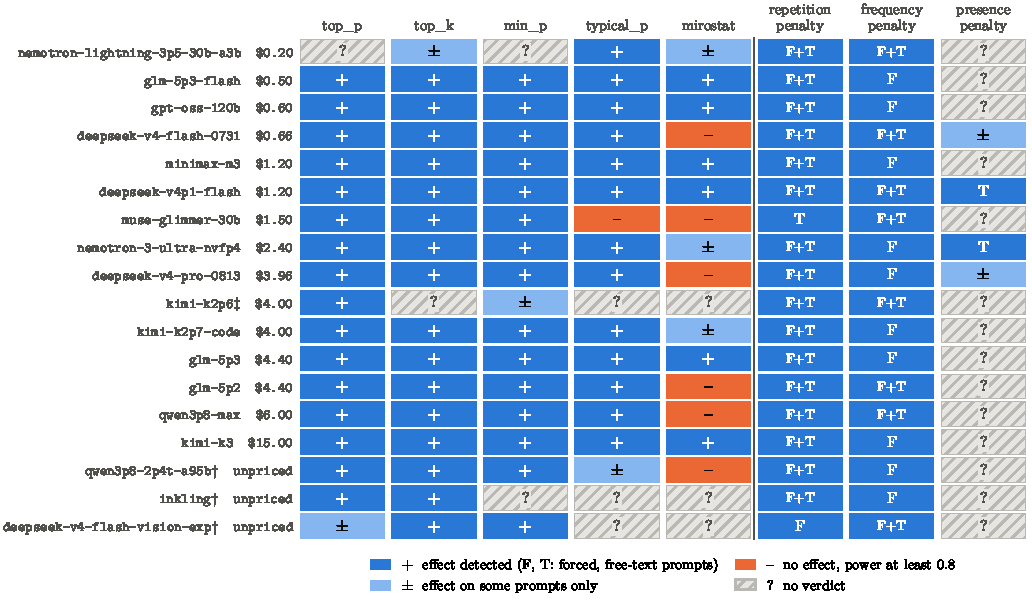
\includegraphics[width=\linewidth]{figures/verdicts.pdf}
\caption{Verdict per model and parameter. Models are ordered by price per million output tokens. For the penalties, F and T mark an effect on the forced-repetition prompt and on the free-text prompts. $\dagger$: 10 completions per arm. $\ddagger$: 40 per arm for \p{top\_p}, \p{top\_k} and \p{min\_p}, 10 for the rest.}
\label{fig:verdicts}
\end{figure}

The API accepted every documented parameter on every model, 162 of 162 (model, parameter) pairs with \p{seed} included. Table~\ref{tab:gap} and Figure~\ref{fig:verdicts} give the verdicts for the eight parameters that shape the sampling distribution. Of 144 cells, 104 show an effect, 7 are mixed, 5 are inert and 28 have no verdict.

The truncation parameters behave as documented wherever the test has power. \p{top\_p}, \p{top\_k} and \p{min\_p} show an effect in 47 of 54 cells and are inert in none. The other seven cells are on four models. On nemotron-lightning-3p5-30b-a3b, temperature 0 leaves most of the open-arm entropy in place, so the test has little power. On kimi-k2p6 the temperature-0 arm is itself highly variable. inkling and deepseek-v4-flash-vision-exp have ten completions per arm.

Mirostat splits the catalogue. It is honoured on six models (glm-5p3-flash, gpt-oss-120b, minimax-m3, deepseek-v4p1-flash, glm-5p3 and kimi-k3) and inert on four others (deepseek-v4-flash-0731, glm-5p2, muse-glimmer-30b and qwen3p8-max). On those four the test had power 1.00 against a greedy-strength effect, and the upper bound on the effect is at most 0.19 of the temperature-0 contrast, below the 0.24 of the weakest model that honours mirostat. Three more models show no effect (deepseek-v4-pro-0813, nemotron-lightning-3p5-30b-a3b and qwen3p8-2p4t-a95b), but there an effect as large as the weakest honoured one cannot be excluded (upper bounds 0.27 to 0.36), so they have no verdict. Every request went to the same endpoint with the same fields, so whether mirostat changes the output depends on the model, and a caller cannot tell which from the documentation or the response. The split runs through model families: deepseek-v4p1-flash honours mirostat and deepseek-v4-flash-0731 does not, and glm-5p3 and glm-5p3-flash honour it and glm-5p2 does not. muse-glimmer-30b also ignores \p{typical\_p} ($p = 0.52$ over four prompts, power 1.00, upper bound 0.10 against a threshold of 0.20) while it honours \p{top\_p}, \p{top\_k} and \p{min\_p}.

A parameter can be applied and still change little. \p{frequency\_penalty}=2.0 changes the forced-repetition output on all 18 models. On the free-text prompts it changes the output distribution on 8 models, is mixed on 2, and has no detectable effect on 8, where the test had at least 0.8 power against the reference contrast. A harness that reports \p{frequency\_penalty}=2.0 reports a setting that is real and that, for short replies on almost half of these models, changes nothing we can detect.

\p{repetition\_penalty}=2.0 shows an effect on all 18 models, on the forced prompt for 17 of them. On three (inkling, qwen3p8-max and qwen3p8-2p4t-a95b) every forced reply with the penalty on is empty, where every reply without it repeats the word. On muse-glimmer-30b the forced reply is unchanged in 39 of 40 calls, yet the penalty changes the free-text output on all four prompts (pooled $p < 0.001$). Calling that model inert on the strength of the forced prompt would have been wrong, and it is the reason a forced null decides only \p{frequency\_penalty}.

\p{presence\_penalty} is the one parameter the design cannot resolve. It shows an effect on two models (deepseek-v4p1-flash and nemotron-3-ultra-nvfp4, both on free text) and is mixed on one. On the forced prompt the repeated word survives the maximum penalty on 16 models, with the two arms identical, and the output does not change on the other two. A penalty of at most 2 logits cannot be expected to overturn a forced token, so these nulls do not separate a parameter that is ignored from one that is applied and too weak to matter. The remaining 15 models have no verdict.

\subsection{Accepted and undocumented}
\label{sec:undoc}

\begin{table}[t]
\centering
\small
\caption{Parameters the API accepts and does not document, on five models. \emph{Accepted} counts requests not rejected with HTTP 400. Collected 22 September 2026.}
\label{tab:undoc}
\begin{tabularx}{\linewidth}{llcX}
\toprule
Parameter & An applied setting must show & Accepted & Result \\
\midrule
\inputrows{generated/table_undoc.tex}
\bottomrule
\end{tabularx}
\end{table}

Table~\ref{tab:undoc} gives the results for the four undocumented parameters. A caller who sets \p{use\_beam\_search} gets HTTP 200, no warning and ordinary sampling. Beam search is deterministic, yet with the parameter set no model returns the same reply to all ten calls at temperature 1.0. The most common reply appears 1 to 6 times in ten, and on four models its count rises by at most two when the parameter is set. \p{skip\_special\_tokens} set to false exposes no end-of-turn marker on any of the five. These nine cells are the case the audit was built to find, a parameter that is accepted, absent from the documentation and without effect. The \p{skip\_special\_tokens} design assumes that an honoured setting renders the terminating token in the text. A stack that drops that token in every case would pass the same test, so those five cells are weaker evidence than the rest.

\p{ignore\_eos} is the mirror case, and for evaluation the worse one. It is undocumented and works on three models. Generation continues past the end-of-turn token to the cap, and the raw control token appears in the returned text (\texttt{cat<|assistant|>We need answer...} on glm-5p3-flash). On a fourth model the control request already ran to the cap, so the test could not decide, and kimi-k3 answers every request that sets the parameter with HTTP 500. Nothing in the reference says the parameter exists.

One documented value was also unreliable. At \p{repetition\_penalty}=2.0, the documented maximum, some requests stalled mid-generation for minutes until the connection dropped. They completed on retry at lower concurrency, so no verdict rests on a stalled request, and the probe now records a request the provider never finishes as an outcome of its own.

\subsection{Temperature-0 decoding is not reproducible}
\label{sec:determinism}

\begin{figure}[t]
\centering
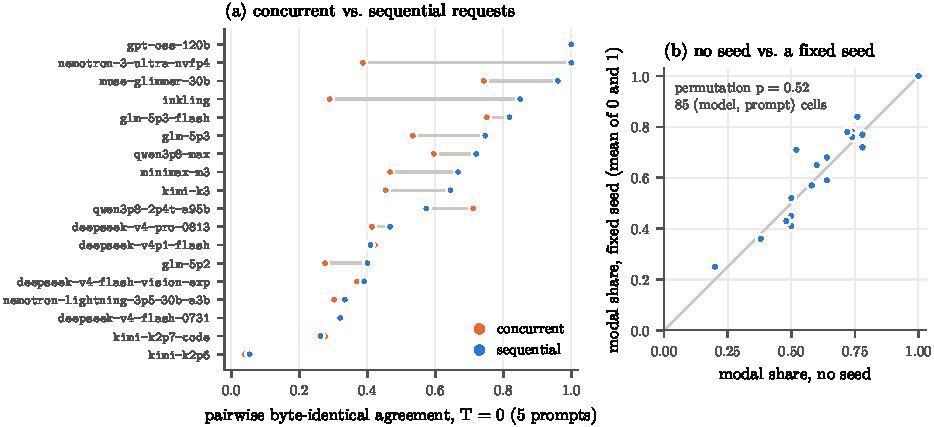
\includegraphics[width=\linewidth]{figures/determinism.pdf}
\caption{Temperature 0. (a) Pairwise agreement of ten identical requests per prompt, averaged over five prompts, when the requests are in flight together and when each waits for the previous response (23 September 2026). (b) Modal share of ten identical requests without a seed and with a fixed seed (mean of \p{seed}=0 and \p{seed}=1), per model, averaged over five prompts. The diagonal is no effect. The permutation test is over the 85 (model, prompt) cells of the 17 nondeterministic models.}
\label{fig:determinism}
\end{figure}

gpt-oss-120b is the only model of the 18 that returns byte-identical output to ten identical temperature-0 requests on all five prompts. On the other 17 the modal share, averaged over prompts, ranges from 20\% (kimi-k2p6) to 78\%. Price does not predict it. kimi-k3, the most expensive model at \$15.00 per million output tokens, reaches 74\%, and glm-5p3-flash at \$0.50 reaches 76\%. On the MATH-500 problem, 7 of 18 models return the same response to all ten requests, and kimi-k2p6 returns its most common response in 2 of 10 (Appendix~\ref{app:determinism}). For such a model a reported greedy accuracy is one draw from a distribution.

Batch composition is a known source of this nondeterminism \citep{he2025defeating}, and a probe that sends its requests together changes the batches they land in. Sent one at a time, two models are fully reproducible (gpt-oss-120b and nemotron-3-ultra-nvfp4). Sent together, only gpt-oss-120b is. Pairwise agreement is higher for sequential requests in 48 of 90 (model, prompt) pairs and lower in 25 (sign test, $p = 0.0095$), and the mean modal share is 70\% sequential against 61\% concurrent. The effect is concentrated (Figure~\ref{fig:determinism}a). Pairwise agreement rises by at least 10 points on 8 models, and nemotron-3-ultra-nvfp4 goes from 39\% pairwise (56\% modal) when concurrent to 100\% when sequential. It falls by 14 points on qwen3p8-2p4t-a95b and does not move on kimi-k2p6, which returns its modal response 22\% of the time either way. Sequential here means sequential from our client. The provider still batches each request with other customers' traffic, which no client controls.

The reference describes \p{seed} as ``Random seed for deterministic sampling.'' Setting one does not make temperature-0 output more reproducible (Figure~\ref{fig:determinism}b). Over the 85 (model, prompt) cells of the 17 nondeterministic models, the modal share with a fixed seed is on average 1.2 points higher than without one (permutation $p = 0.52$). Of 73 cells that are not reproducible without a seed, a fixed seed makes 10 reproducible. The reverse happens at a similar rate: of 70 cells not reproducible with \p{seed}=0, 7 are reproducible without a seed or with \p{seed}=1. This result concerns the documented promise. The design cannot tell whether the seed would fix the random draws at a temperature above 0. It does show that a caller who writes \p{seed}=0 into a temperature-0 configuration, and ``reproducible'' into a paper, gets no reproducibility from the seed.

\subsection{How stable the verdicts are}
\label{sec:robust}

\paragraph{Multiplicity.} Holm's procedure runs within each collection run. Under one correction over all 182 tests in the audit (144 pooled free-text tests and 38 forced-prompt tests with a $p$-value), 5 of the 104 honoured cells lose significance: \p{top\_p} on inkling and on kimi-k2p6, \p{typical\_p} on kimi-k2p7-code, and the two effects of \p{presence\_penalty}. The five inert cells are unaffected.

\paragraph{The null threshold.} A cell is inert when its Holm-adjusted $p$ exceeds 0.05 and both the power criterion and the effect bound hold. The $p$ threshold suits a claim of an effect and is lenient for a claim of absence. Requiring the unadjusted $p$ to exceed 0.05 as well moves no cell, since the five inert cells have unadjusted $p$ between 0.13 and 0.65. The effect bound is the stricter rule. Without it mirostat would count as inert on seven models, among them deepseek-v4-pro-0813 with an unadjusted $p$ of 0.019.

\paragraph{What an effect shows.} A detected effect shows that the output depends on the parameter. It does not show that the sampler applied the parameter as documented, since a field could, for example, send a request to a different replica or kernel configuration. For \p{top\_k}=1 the documented mechanism has an exact signature. The tight arm is then greedy decoding and should be distributed like the temperature-0 arm of the same model and prompt. The two differ (TV permutation test, $p < 0.05$) on 6 of 62 informative (model, prompt) pairs. For \p{top\_p}=0.01 and \p{min\_p}=0.9 they differ more often, on 18 and 24 of 63 pairs. On gpt-oss-120b, which is deterministic at temperature 0, the \p{top\_p}=0.01 arm splits evenly between two responses to the word-problem prompt. These two settings narrow the distribution without reducing it to greedy decoding, and a black-box test cannot say whether tie handling, numerics or the serving path is the reason. Mirostat, \p{typical\_p} and the penalties have no signature beyond the direction of the effect and, for \p{frequency\_penalty}, the broken forced repetition. An inert verdict does not depend on this question, because it rests on the absence of any change in the output.

\paragraph{The aggregation rule.} An earlier version of the analysis combined prompts by majority vote, which has no stated error rate. Over all collection runs, including runs later superseded by larger ones, the two rules agree on 132 of 211 aggregates. Of the 79 disagreements, 55 are cells the vote left undetermined that pooling resolves, 11 become mixed, 4 move from mixed to an effect, and 9 reverse a definite verdict. All nine go from the vote's ``no effect'' to an effect. None goes the other way.

\paragraph{Drift and thin rows.} The same cell collected on two dates can differ. On minimax-m3 and the word-problem prompt, 11 of 40 temperature-0 completions were distinct in the first run (collected on or before 17 September) and 20 of 40 when collected again on 20 and 21 September. The three models without a published price ran at 10 completions per arm, where the bootstrap estimates of power and of the effect bound are optimistic. The effect bound is also widest there, and it is the reason qwen3p8-2p4t-a95b, whose mirostat test found nothing, has no verdict.

\section{What an ignored parameter does to an evaluation}
\label{sec:consequences}

The audit asks whether parameters are applied. This section shows, on real generations, how the answer and two related decisions in an evaluation harness reach the numbers a decoding study reports. The corpus is small (ten MATH-500 problems, five replicates, three or four models), and the magnitudes illustrate the mechanism. They are not estimates of its size.

\paragraph{An ignored parameter creates an interaction.} Take two cells of a decoding grid, \{temperature 1.0, \p{min\_p}=0.05\} and \{temperature 1.0, \p{top\_p}=1.0\}. For a model whose provider applies \p{min\_p} they are two conditions. For a model whose provider ignores it they are one condition run twice. A grid that mixes the two kinds of model, which Section~\ref{sec:gap} shows can happen behind one API, contains a contrast that is real for some models and zero for others, and a two-way variance decomposition books the difference as a model $\times$ sampler interaction. We built both cases from real generations on three models (300 generations, collected on 22 September 2026): a genuine \p{min\_p} cell, and five extra replicates of the \p{top\_p}=1.0 cell, which is what an ignoring provider returns for the \p{min\_p} request. With every model's provider applying \p{min\_p}, the interaction accounts for 7.9\% of the variance. With one model's provider ignoring it, the share is 3.3\% to 5.6\%, depending on the model. With all three ignoring it, the share is 1.0\%, and with all but one ignoring it, 1.7\% to 3.4\%. Each figure is a correct analysis of a correctly collected accuracy table, and the table carries no trace of which case produced it.

\paragraph{Unparseable responses are a third outcome.} On 1{,}000 generations (four models and five sampler settings, collected in August 2026), minimax-m3 gives no parseable answer in 10\% of responses at temperature 0 and 18\% at temperature 1.0, with the three intermediate settings at 12\% to 16\%. The other three models give none. All 35 such responses stopped at the 8{,}192-token cap in the middle of their reasoning. Scored as incorrect, they give minimax-m3 a temperature effect of 0.06 in accuracy (0.88 at temperature 0 and 0.82 at 1.0). Among the responses it finishes, its accuracy is 0.98 to 1.00 at every setting, the highest of the four models. The scoring rule alone reverses 12 of the 30 pairwise model comparisons across sampler settings. Folding unparseable responses into ``incorrect'' is a choice that falls on one model and grows with temperature, so it belongs in a separate column of the results.

\paragraph{The grader has to be checked by hand.} Labelling a stratified sample of 50 responses by hand exposed five defects in the exact-match grader. One was a fallback that took the last number in a truncated response, and it once scored a response that never stated an answer as correct. Truncation is common: in the 500 generations the sample was drawn from, 10\% to 13\% of responses ran out of tokens at every sampler setting. A grader whose error rate depends on the sampler would enter a decoding study as a sampler effect. After the fixes the grader agrees with the hand labels on all 50 items of a second sample.

\section{Discussion}

\paragraph{For evaluations on hosted APIs.} Each result above suggests a practice. Probe every parameter a study varies, on every model, at settings extreme enough that an honoured parameter must show, since acceptance proves nothing and the answer differs between models behind one API (Section~\ref{sec:gap}). Treat a temperature-0 result as a draw from a distribution, report its spread, and record how many requests were in flight (Section~\ref{sec:determinism}). Do not rely on a seed for reproducibility without measuring it. Score unparseable responses as a third outcome, and check the grader by hand on a sample weighted toward rare cases (Section~\ref{sec:consequences}).

\paragraph{For providers.} A validator that rejects unknown fields, as this one does for 15 names from other stacks, lets a caller trust that an accepted field is known to the server. That trust fails when a field is accepted and dropped, as \p{use\_beam\_search} is, or accepted and applied on some models only, as mirostat is. An error or a warning for a parameter that a model's serving path ignores would close the gap, and so would documentation per model.

\paragraph{For studies of decoding variance.} This instrument was built for a study that splits the variance of benchmark accuracy into model, sampler and interaction components. We do not report that study, and the reason is not compute. A variance component estimated from $k$ factor levels has a relative standard error of about $\sqrt{2/(k-1)}$, which is 100\% at three levels and 58\% at seven. In a simulation of the planned grid (three models, seven sampler settings, five replicates), an interval for the ratio of sampler to model variance clears a threshold of 0.1 in only 57\% of simulated grids when the two components are equal (Appendix~\ref{app:levels}). More problems and more replicates do not change this. More model levels do, and a band of similar models on one provider does not contain enough of them. A count over observed cells, such as how often the ranking of two models flips when only the sampler changes, needs no extrapolation from a few levels and is the more testable headline for such a study.

\section{Limitations}

\paragraph{One provider.} All 18 models sit behind one API. Mirostat shows that compliance can differ between models there, but whether the same model complies differently at two providers is not answered here. The probes reach other providers through adapters, and the documentation of six other providers is already transcribed. The extension needs API access and budget. It does not need new code.

\paragraph{Short replies and exact matches.} The test compares exact strings of short replies. It detects whether a parameter changes the output distribution. It does not measure how much a parameter changes long outputs or task accuracy, and a parameter that matters only in long generations can look inert here, as the free-text results for the penalties show.

\paragraph{Behaviour, not mechanism.} Honoured is a behavioural verdict. Except for \p{top\_k}=1, whose tight arm matches greedy decoding, the audit cannot tell a sampler that applies a parameter from a serving path that changes in some other way when the field is set.

\paragraph{The power reference and the effect bound.} Inert rests on power against a greedy-strength effect and on a bootstrap bound against the weakest honoured effect of the same parameter. Both treat the observed arms as the truth, which is optimistic at 10 completions per arm, and the weakest honoured effect is the estimate from a single model.

\paragraph{The seed.} We test the documented promise at temperature 0 only. Whether the seed fixes the random draws at higher temperatures, as a working seed would, is untested.

\paragraph{Undocumented parameters.} The \p{skip\_special\_tokens} design assumes that an honoured setting renders the end-of-turn token, and \p{best\_of} could not be tested from outside.

\paragraph{Drift and load.} Provider behaviour changed within days (Section~\ref{sec:robust}) and models were withdrawn during the study, so every result is a dated observation. The concurrency comparison controls only this client's load.

\subsubsection*{Broader impact statement}

This paper audits a commercial service and names it, its models and its documentation. The findings describe behaviour observed between 17 and 23 September 2026 and may not hold later. They do not show why a parameter is ignored, or that anyone intended it. The effect we expect is on evaluation practice: results that depend on decoding parameters or seeds served by a hosted API can be checked with the released instrument before they are compared. The released completions are unfiltered model output, and at high temperature some contain invented text, including strings formatted as email addresses. No human subjects were involved.

\subsubsection*{Reproducibility statement}

The supplementary material contains the instrument, its test suite, and every committed record. Every table and figure in this paper regenerates from those records without an API key or network access (\texttt{make numbers} writes a table that traces each number in the text to its source file, and \texttt{scripts/paper\_assets.py} draws the figures and tables). The records keep every completion behind every parameter verdict, so a verdict can be recomputed under a changed test. For the determinism and undocumented-parameter probes the records keep per-condition summaries (modal share, number of distinct responses and the modal response). The raw responses of those probes sit in the response cache, which is not part of the supplementary material.

\bibliographystyle{tmlr}
\bibliography{refs}

\appendix
\raggedbottom

\section{Models and collection dates}
\label{app:models}

\begin{table}[H]
\centering
\small
\caption{The 18 chat models of the serverless catalogue, with the published price per million tokens (read 20 September 2026), completions per arm, and the collection window of the parameter and determinism probes (the concurrency run of 23 September not included). $^{a}$40 per arm for \p{top\_p}, \p{top\_k} and \p{min\_p}, 10 for the other parameters.}
\label{tab:models}
\begin{tabular}{lrrcc}
\toprule
Model & Input \$/M & Output \$/M & Per arm & Collected (2026) \\
\midrule
\inputrows{generated/table_models.tex}
\bottomrule
\end{tabular}
\end{table}

\section{Prompts}
\label{app:prompts}

The four free-text prompts of the distinguishability test, each sent as the only user message:
\begin{itemize}
\item \emph{word problem}: ``Write a one-sentence arithmetic word problem suitable for a ten-year-old. Reply with the problem only.''
\item \emph{sentence}: ``Write one short sentence about anything at all. Reply with the sentence only.''
\item \emph{opener}: ``Write the opening three words of a story. Reply with those three words only.''
\item \emph{question}: ``Ask one question about anything. Reply with the question only.''
\end{itemize}
The forced-repetition prompt for the penalties: ``Repeat the word `yes' twenty times, separated by spaces. Reply with only that.''

The undocumented-parameter tests use ``Reply with the single word: cat'' for \p{ignore\_eos}, \p{skip\_special\_tokens} and \p{best\_of}, and the \emph{sentence} prompt for \p{use\_beam\_search}.

The determinism probe adds MATH-500 problem \texttt{test/algebra/1004} under the evaluation prompt ``Solve the problem. Reason step by step, then give the final answer on its own last line in the form: Answer: <answer>'', followed by the problem.

The prompts were fixed on 11 September 2026 by measuring open-arm entropy (temperature 1.0, 20 samples) on three models. The three rejected candidates asked for a fact about numbers, an integer between 1 and 1000, and the name of a city.

\section{Cells without a clean effect}
\label{app:cells}

\begin{table}[H]
\centering
\scriptsize
\caption{The 40 cells of Table~\ref{tab:gap} that are not honoured. Pr.: prompts pooled. $p$: pooled stratified test, unadjusted. Holm run: adjusted within the collection run, the basis of the verdict. Holm all: one correction over all 182 tests. Power: estimated power against the greedy-strength reference. Effect: entropy removed as a fraction of what temperature 0 removes, pooled over prompts, and its 95\% bootstrap upper bound (truncation parameters). A null is inert only if the bound lies below 0.24 for mirostat and 0.20 for \p{typical\_p}. Forced: the forced-prompt result for a penalty (\textminus: no change, ?: both arms the same constant). Every cell, including the 104 honoured ones, is in \texttt{paper/generated/cells.csv}.}
\label{tab:cells}
\setlength{\tabcolsep}{2.4pt}
\begin{tabular}{llrrrrrrrrcl}
\toprule
Model & Parameter & $n$ & Pr. & $p$ & Holm run & Holm all & Power & Effect & Bound & Forced & Verdict \\
\midrule
\inputrows{generated/table_cells.tex}
\bottomrule
\end{tabular}
\end{table}

\section{Determinism per model}
\label{app:determinism}

\begin{table}[H]
\centering
\small
\caption{Temperature 0, per model. Modal share of ten identical requests (five in flight), averaged over five prompts, without a seed and with \p{seed}=0 and \p{seed}=1 (17 and 20 September 2026). MATH-500: responses equal to the modal response, no seed. Pairwise agreement and prompts fully reproduced, with the ten requests in flight together (conc.) and sent one at a time (seq.), on 23 September 2026.}
\label{tab:determinism}
\setlength{\tabcolsep}{4.5pt}
\begin{tabular}{lccccccccc}
\toprule
 & \multicolumn{3}{c}{Modal share} & & \multicolumn{2}{c}{Pairwise} & \multicolumn{2}{c}{Prompts reproduced} \\
\cmidrule(lr){2-4}\cmidrule(lr){6-7}\cmidrule(lr){8-9}
Model & no seed & seed 0 & seed 1 & MATH-500 & conc. & seq. & conc. & seq. \\
\midrule
\inputrows{generated/table_determinism.tex}
\bottomrule
\end{tabular}
\end{table}

\section{Few model levels cannot test a variance ratio}
\label{app:levels}

\begin{table}[H]
\centering
\small
\caption{Simulated grids of three models, seven sampler settings and five replicates, 40 grids per row, with variance components calibrated to the pilot accuracies. \emph{Point}: the estimated ratio of sampler to model variance exceeds 0.1. \emph{Interval}: the lower bound of an interval that resamples factor levels exceeds 0.1. Produced by \texttt{scripts/power\_check.py}.}
\label{tab:levels}
\begin{tabular}{ccc}
\toprule
True ratio & Point clears 0.1 & Interval clears 0.1 \\
\midrule
0.05 & 40\% & 0\% \\
0.10 & 52\% & 0\% \\
0.25 & 72\% & 10\% \\
0.50 & 82\% & 35\% \\
1.00 & 95\% & 57\% \\
2.00 & 98\% & 78\% \\
\bottomrule
\end{tabular}
\end{table}

\section{What the reference documents}
\label{app:docs}

The Fireworks AI chat completions reference \citep{fireworks2026reference}, read on 22 September 2026, describes: \p{temperature} (range 0 to 2), \p{top\_p} as nucleus sampling over the tokens holding \p{top\_p} of the probability mass (0 to 1), \p{top\_k} as filtering to the $k$ most probable tokens with the mass renormalised (0 to 100, and the API rejects 200), \p{min\_p} as keeping only tokens whose probability is at least \p{min\_p} (0 to 1), \p{typical\_p} as keeping the most typical tokens up to that cumulative probability (0 to 1), \p{mirostat\_target} as the target perplexity of the mirostat algorithm and \p{mirostat\_lr} as its learning rate, \p{repetition\_penalty} as no penalty at 1.0 and a penalty on repetition above 1.0 (0 to 2), \p{frequency\_penalty} and \p{presence\_penalty} as penalties on tokens by their frequency and by their presence in the text so far ($-2$ to 2), and \p{seed} as a ``Random seed for deterministic sampling.'' The reference describes \p{min\_p} as an absolute threshold, where the original definition \citep{nguyen2025minp} scales it by the probability of the most likely token. Under either reading \p{min\_p}=0.9 keeps at most the most likely token and its near-ties. The full transcription, with the wording of each entry, is in \texttt{samplerconfound/documented.py}.

\end{document}
